\documentclass[10pt]{extarticle}
% (1) Encoding, Fonts, and Layout
\usepackage[T1]{fontenc}
\usepackage{lmodern}
\usepackage[margin=1in]{geometry}


% (2) Common Packages
\usepackage{amsmath, amssymb, amsthm}
\usepackage{xcolor}
\usepackage{caption}
\usepackage{tikz}
\usepackage{pgfplots}
\pgfplotsset{compat=newest}
\usepackage{etoolbox}
\usepackage{tikz-3dplot}
\tdplotsetmaincoords{75}{120}
\usepackage[inline]{enumitem}
\usepackage{bookmark}
\usepackage{mathtools}
\usepackage{subcaption} % For subfigures
\usepackage[normalem]{ulem} % For better underline commands

% Micro-typography
\usepackage{microtype}

% Patching pgfplots warning
\makeatletter
\patchcmd{\pgfplots@applistXXpushback@smallbuf}{\pgfplots@error}{\pgfplots@warning}{}{}
\makeatother

% (3) tcolorbox and Theorem Libraries
\usepackage{tcolorbox}
\tcbuselibrary{theorems}

% (4) Define Colors
\definecolor{custom_green}{HTML}{a3be8c}
\definecolor{custom_red}{HTML}{dc322f}
\definecolor{custom_blue}{HTML}{268bd2}
\definecolor{custom_purple}{HTML}{b48ead}

\definecolor{base}{HTML}{eceff4}
\definecolor{gray1}{HTML}{e5e9f0}
\definecolor{gray2}{HTML}{d8dee9}
\definecolor{gray3}{HTML}{2e3440}
\pagecolor{base}

% (5) Custom tcolorbox Environments
\newtcolorbox{definitionbox}[1][]{
    title=\textbf{Definition} {#1},
    fonttitle=\bfseries\boldmath,
    arc=0mm,
    bottomtitle=0.5mm,
    boxrule=0mm,
    colbacktitle=gray2,
    colback=gray1,
    coltitle=gray3,
    coltext=gray3,
    left=2.5mm,
    leftrule=1mm,
    rightrule=1mm,
    right=3.5mm,
    toptitle=0.75mm,
    colframe=custom_red,
}

\newtcolorbox{proofbox}{
    title=\textbf{Proof},
    fonttitle=\bfseries\boldmath,
    arc=0mm,
    bottomtitle=0.5mm,
    boxrule=0mm,
    colbacktitle=gray2,
    colback=gray1,
    coltitle=gray3,
    left=2.5mm,
    leftrule=1mm,
    rightrule=1mm,
    right=3.5mm,
    toptitle=0.75mm,
    colframe=custom_blue,
    coltext=gray3,
}

\newtcolorbox{theorembox}[1][]{
    title=\textbf{Theorem} {#1},
    fonttitle=\bfseries\boldmath,
    arc=0mm,
    bottomtitle=0.5mm,
    boxrule=0mm,
    colbacktitle=gray2,
    colback=gray1,
    coltitle=gray3,
    left=2.5mm,
    leftrule=1mm,
    rightrule=1mm,
    right=3.5mm,
    toptitle=0.75mm,
    colframe=custom_green,
    coltext=gray3
}

\newtcolorbox{notebox}{
    title=\textbf{Note},
    fonttitle=\bfseries\boldmath,
    arc=0mm,
    bottomtitle=0.5mm,
    boxrule=0mm,
    colbacktitle=gray2,
    coltitle=gray3,
    left=2.5mm,
    leftrule=1mm,
    rightrule=1mm,
    right=3.5mm,
    toptitle=0.75mm,
    colframe=custom_blue,
    coltext=gray3
}

\newtcolorbox{examplebox}[1][]{
    title=\textbf{Example} {#1},
    fonttitle=\bfseries\boldmath,
    arc=0mm,
    bottomtitle=0.5mm,
    boxrule=0mm,
    colbacktitle=gray2,
    colback=gray1,
    coltitle=gray3,
    left=2.5mm,
    leftrule=1mm,
    rightrule=1mm,
    right=3.5mm,
    toptitle=0.75mm,
    colframe=gray3,
    fontupper=\footnotesize,
    coltext=gray3
}

% (6) Theorem Environments
\theoremstyle{definition}
\newtheorem{definition}{Definition}[section]
\newtheorem{example}[definition]{Example}

\theoremstyle{plain}
\newtheorem{theorem}[definition]{Theorem}

% (7) Hyperlinks
\usepackage{hyperref}
\hypersetup{
    colorlinks=true,    % Use colored text for links
    linkcolor=custom_red,      % Set link text color to red
    pdfborder={0 0 0}   % Remove the default box around links
}

% macros.tex
\newcommand{\intinf}{\int_0^{\infty}} % Integral from 0 to infinity
\newcommand{\diff}[2]{\frac{d#1}{d#2}} % Derivative


\usepackage[svgnames]{xcolor}
\usepackage{listings}


\title{
Robert Davidson \\
\textbf{ST1112: Statistics}
}
\author{
70\% Exam\\
30\% Continuous Assessment (3 parts)
}
\date{}       % Optional: Add date if desired
%--------------------------------------------------------
% Document
%--------------------------------------------------------
\begin{document}
\maketitle
\pagebreak

\tableofcontents
\pagebreak

\section{Inferential Statistics - Interval Estimation}
The ultimate goal in statistical inference is to estimate population parameters (like the mean $\mu$) based on sample statistics (like the sample mean $\bar{X}$).
\subsection{Probability vs Statistics}
\begin{itemize}
    \item \textbf{Probability} deals with known underlying processes: one starts with a model (like proportion of red vs. green jelly beans in a jar) and computes probability of specific outcomes
    \item \textbf{Statistics} works in reverse: one observes outcomes (sample data) and attempts to infer the underlying process or population parameters (e.g. proportion of red jellybeans)
\end{itemize}
\subsection{Definitions and Concepts}

\begin{definitionbox}{Population}{}
    A \textbf{population} is the complete set of items (or individuals) of interest.
\end{definitionbox}

\begin{definitionbox}{Sample}{}
    A \textbf{sample} is a subset of that population, intended to represent the population\\

    For example the sample mean $\bar{X}$ is an estimate of the population mean $\mu$.
\end{definitionbox}

\begin{definitionbox}{Population Mean ($\mu$)}{}
    $\mu$ represents the central tendency of a population distribution.
    $$\mu = \frac{1}{N} \sum_{i=1}^{N} x_i$$
    where $N$ is the population size and $x_i$ are the individual values in the population.\\

    $\mu$ is sometimes called the expected value or average.
\end{definitionbox}

\begin{definitionbox}{Population standard deviation ($\sigma$)}{}
    $\sigma$ measures the dispersion or spread of values around the mean in a population.
    $$\sigma = \sqrt{\frac{1}{N} \sum_{i=1}^{N} (x_i - \mu)^2}$$
    where $N$ is the population size and $x_i$ are the individual values in the population.\\
\end{definitionbox}

\begin{conceptbox}{Sampling Variation}{}
    When we take multiple samples from the same population, each sample's mean $\bar{X}$ will be different. This is variability is called \textbf{sampling variation}. \\

    Larger sample sizes tend to reduce this variation, that is as $n$ gros, the sample mean $\bar{X}$ becomes a better estimate of the population mean $\mu$.
\end{conceptbox}
\begin{conceptbox}{Sampling Distributions}{}
    The sample mean itself is a \textbf{random variable} because different samples yield different mean values.\\

    The distribution of all possible sample means (of a given sample size $n$) is called the \textbf{sampling distribution} of the sample mean ($\bar{X}$).
\end{conceptbox}

\begin{definitionbox}{Expected Value of the Sample Mean}{}
    $$E(\bar{X}) = \mu$$
    This means if you averaged all possible sample means, you would get the population mean $\mu$.
\end{definitionbox}
\begin{definitionbox}{Standard Error of the Mean}{}
    $$SE = SD(\bar{X}) = \frac{\sigma}{\sqrt{n}}$$
    where $\sigma$ is the population standard deviation and $n$ is the sample size.\\

    This value is called the \textbf{standard error} of the mean and measures how much the sample mean $\bar{X}$ fluctuates around the population mean $\mu$.
\end{definitionbox}

\begin{definitionbox}{Central Limit Theorem}{}
    $$\bar{X} \sim N\left(\mu, \frac{\sigma^m}{n}\right)$$
    where $\bar{X}$ is the sample mean, $\mu$ is the population mean, and $\sigma$ is the population standard deviation.\\

    The \textbf{Central Limit Theorem} states that the sampling distribution of the sample mean $\bar{X}$ (the distribution of all sample means)  approaches a normal distribution as the sample size $n$ increases, \textbf{regardless of the shape of the population distribution.}\\

    This means that for large enough sample sizes, we can use the normal distribution to make inferences about the population mean $\mu$. \\

    \textbf{Practically}, many apply the rule of thumb $n \geq 30$ to treat $\bar{X}$ as normally distributed.
\end{definitionbox}


\begin{definitionbox}{Unbiased Estimators}{}
    We say a statistic $T$ is an \textbf{unbiased estimator} of a population parameter $\theta$,  if $E(T) = \theta$.\\

    For example, the sample mean $\bar{X}$ is an unbiased estimator of the population mean $\mu$ because $E(\bar{X}) = \mu$.\\

    The sample standard deviation $s$ (using Bessel's correction, dividing by multiplying by $\frac{1}{n-1}$ rather than $\frac{1}{N}$) is an unbiased estimator of the population standard deviation $\sigma$.
\end{definitionbox}

\subsection{Example}
\begin{examplebox}{Weekly rent}{}
    If a population mean rent is $\mu = 225$, with $\sigma = 25$ for a population sample size $n = 30$, the sample distribution of the sample mean is approximately:
    $$\bar{X} \sim N\left(225, \frac{25^2}{30}\right)$$
    This lets us compute probabilities for specific sample mean ranges using the normal distribution (e.g. $P(\bar{X} < 220)$).
\end{examplebox}
\subsection{Recap}
A \textbf{sample statistic} (e.g. the sample mean $\bar{X}$) varies from one sample to another. Understanding this variation (and quantifying it via the standard error) is crucial for knowing how precise (or imprecise) an estimate really is. \\[2ex]
If we have a large sample size $n$ from a population with mean $\mu$ and standard deviation $\sigma$, then our sample distribution of the sample mean $\bar{X}$ is approximately normal:
$$\bar{X} \sim N\left(\mu, \frac{\sigma^2}{n}\right)$$
In practice, for $n \geq 30$, $\bar{X}$ can be treated as normally distributed even if the original population is not strictly normal.

\section{Confidence Intervals}

\subsection{Confidence Intervals}
\begin{conceptbox}{Why confidence intervals?}{}
    Why do we need confidence intervals, instead of a single point estimate, like the sample mean $\bar{X}$? \\

    A confidence interval provides a range of plausible values for the population parameter (e.g. $\mu$) based on the sample data. \\

    \textbf{Analogy:}  Using a single point estimate is like trying to catch a fish wih a spear; your aim may not be perfect. Using a confidence interval is like using a net; we have a better chance of "catching" (capturing) the true population parameter.
\end{conceptbox}
\begin{definitionbox}{Confidence Interval}{}
    $$\bar{X} \pm (\text{critical value}) \times SE(\bar{X})$$
    where $SE(\bar{X}) = \frac{\sigma}{\sqrt{n}}$ is the standard error of the sample mean, $\pm$ is the margin of error. \\
    The general formula for a desired confidence level 100(1- $\alpha$)\% is:
    $$\bar{X} \pm z_{\alpha/2} \times \frac{\sigma}{\sqrt{n}}$$
    where $z_{\alpha/2}$ is the critical value from the standard normal distribution.
\end{definitionbox}
\noindent\textbf{Interpretation}: \\
If we repeat the sampling process many times and construct confidence intervals from each sample, then approximately $100 \times (1 - \alpha)\%$ of those intervals will contain the true population parameter $\mu$.\\
In other words, you do not say \emph{"there is a 95\% chance that $\mu$ lies in my interval"}. Rather we say, \textbf{"on repeated sampling 95\% of such intervals will contain the true population mean $\mu$."}


\begin{definitionbox}{Critical Values}{}
    The \textbf{critical value} is a z-score that corresponds to the desired confidence level. \\[2ex]
    For example, for a 95\% confidence level, the critical value is $Z_{\alpha/2} = 1.96$ (where $\alpha = 0.05$).
    This means that 95\% of the area under the normal curve lies within $1.96$ standard deviations of the mean. \\[2ex]
    \begin{center}
        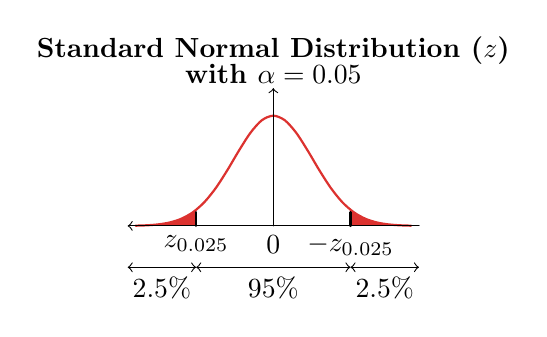
\begin{tikzpicture}[
                domain=-1:1,
                xscale=-0.5,
                yscale=3.5,
                smooth,
                line cap=round,
                line join=round,
            ]
            % Define critical z values
            \def\zcrit{1.96}

            % Fill left tail area (2.5%)
            \fill[custom_red] (-3.5,0) -- plot[domain=-3.5:-\zcrit] (\x, {0.4*exp(-(\x)^2/2)}) -- (-\zcrit,0) -- cycle;

            % Fill right tail area (2.5%)
            \fill[custom_red] (3.5,0) -- plot[domain=3.5:\zcrit] (\x, {0.4*exp(-(\x)^2/2)}) -- (\zcrit,0) -- cycle;

            % Draw the normal distribution curve
            \draw[thick, custom_red] plot[domain=-3.5:3.5] (\x, {0.4*exp(-(\x)^2/2)});

            % Mark the critical values
            \draw[thick] (-\zcrit,0) -- (-\zcrit,0.05);
            \node[below] at (-\zcrit,0) {$-z_{0.025}$};
            \draw[thick] (\zcrit,0) -- (\zcrit,0.05);
            \node[below] at (\zcrit,0) {$z_{0.025}$};

            \draw[<->] (-\zcrit, -0.15) -- (\zcrit, -0.15) node[midway, below] {$95\%$};
            \draw[<->] (-\zcrit, -0.15) -- (-3.7, -0.15) node[midway, below] {$2.5\%$};
            \draw[<->] (\zcrit, -0.15) -- (3.7, -0.15) node[midway, below] {$2.5\%$};


            % Draw horizontal axis
            \draw[->] (-3.7,0) -- (3.7,0) node[right] {};
            % Draw vertical axis
            \draw[->] (0,0) -- (0,0.5) node[above] {};
            % Mark the center
            \node[below] at (0,0) {$0$};
            % Title
            \node[above] at (0,0.55) {\textbf{Standard Normal Distribution ($z$)}};
            \node at (0,0.55) {\textbf{with $\alpha = 0.05$}};
        \end{tikzpicture}
    \end{center}
\end{definitionbox}

\begin{examplebox}{Find crtitical value for the 95\% CI}{}
    For a confidence interval of 95\%, we want to find the z-score that leaves 2.5\% in each tail of the normal distribution.\\
    We want to find the $z$-value where the cumulative area )from the left up to that $z-score$) is $1 - 0.025 = 0.975$.\\
    We look in the $z$-tables for the value closest to $0.975$ and read the row and column headers to find the $z$-value.\\
    The $z$-value is $1.96$.\\
\end{examplebox}

\begin{examplebox}{Find the 95\% confidence interval for the population mean $\mu$ given}{}
    A dataset of 103 students, of whom 71 pay rent, was used to estimate the average weekly rent $\mu$.
    \begin{itemize}
        \item \textbf{Point estimate}: the sample mean $\bar{X} \approx 546.239$.
        \item \textbf{Sample standard deviation}: $s \approx 187.862$.
        \item \textbf{Sample size}: $n = 71$.
    \end{itemize}
    Confidence Interval is given by:
    $$\bar{X} \pm z_{\alpha/2} \times \frac{s}{\sqrt{n}}\Rightarrow 546.239 \pm 1.96 \times \frac{187.862}{\sqrt{71}}$$
    where $z_{\alpha/2} = 1.96$ for a 95\% confidence level.The resulting confidence interval is:
    $$(502.541, 589.938)$$
    \textbf{Interpretation}: We are 95\% confident that the true mean weekly rent for all NUI Galway students (population) is roughly 503 to 590 euros.
\end{examplebox}
\subsection{Higher Confidence Levels means Wider Intervals}
\begin{itemize}
    \item To achieve a \textbf{higher confidence level}, we need to increase the critical value $z_{\alpha/2}$, which in turn increases the margin of error.
    \item This results in a wider confidence interval, which means we are more certain that the true population parameter lies within that interval.
    \item Conversely a \textbf{lower confidence level} results in a smaller critical value, leading to a narrower confidence interval.
\end{itemize}
\pagebreak
\subsection{t-Distribution}
\begin{conceptbox}{Why the $t-$distribution}{}
    When the sample size is small ($n < 30$) and the population standard deviation $\sigma$ is unknown, simply substituting the sample standard deviation $s$ no longer suffices because the standard error is itself estimated with more uncertainty.\\[2ex]
    The $\textbf{t-distributution has thicker}$ tails than the normal distributution. This extra "fatness" in the tails accounts for the additional uncertainty in using $s$ instead of $\sigma$.
    \begin{center}
        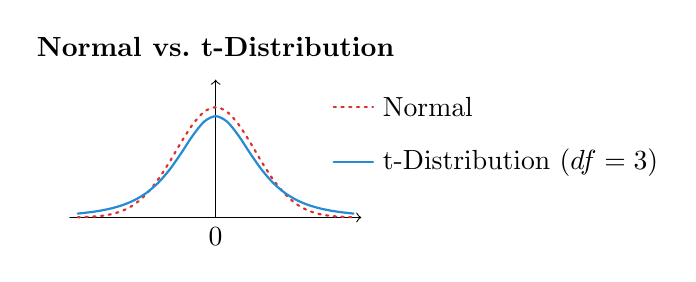
\begin{tikzpicture}[
            domain=-3.5:3.5,
            xscale=0.5,
            yscale=3.5,
            smooth,
            line cap=round,
            line join=round
        ]
            % Draw axes
            \draw[->] (-3.7,0) -- (3.7,0) node[right] {$$};
            \draw[->] (0,0) -- (0,0.5) node[above] {$$};
            \node[below] at (0,0) {$0$};
        
            % Plot the Normal Distribution (dotted red)
            \draw[dotted, thick, custom_red] plot (\x, {0.4*exp(-(\x)^2/2)});
        
            % Plot the t-Distribution (solid blue) for df = 5.
            % The t-density: f(t) = (8/(3*pi*sqrt(5)))*(1+t^2/5)^(-3)
            \draw[thick, custom_blue] plot (\x, {(2/(3.14159*sqrt(3)))*((1+(\x)^2/3)^(-2))});
        
            % Title and legend
            \node[above] at (0,0.55) {\textbf{Normal vs.\ t-Distribution}};
        
            % Legend (placed at the top-right)
            \begin{scope}[shift={(3,0.4)}]
                \draw[dotted, thick, custom_red] (0,0) -- (1,0);
                \node[right] at (1,0) {Normal};
                \draw[thick, custom_blue] (0,-0.2) -- (1,-0.2);
                \node[right] at (1,-0.2) {t-Distribution ($df=3$)};
            \end{scope}
        \end{tikzpicture}        
    \end{center}
\end{conceptbox}
\vfill
\begin{conceptbox}{Degrees of Freedom (df)}{}
    A t-distribution is characterized by its degrees of freedom, where 
    $$df = n - 1 \quad \text{for a sample mean}$$
    As the sample size $n$ increases, the t-distribution approaches the standard normal distribution.\\
    For example, for $n = 30$, $df = 29$ and the t-distribution is very close to the normal distribution.\\
\end{conceptbox}
\vfill
\begin{definitionbox}{Confidece Intervals (t-based)}{}
    $$\bar{X} \pm t_{\alpha/2, df} \times \frac{s}{\sqrt{n}}$$
    where $t_{\alpha/2, df}$ is the critical value from the t-distribution with $df = n - 1$ degrees of freedom - or from a function like \texttt{qt()} in R.\\

    \textbf{Assumption}: The population itself should be approximately normally distributed when using t-based methods for small sample sizes.
\end{definitionbox}
\vfill
\begin{examplebox}{Finding t-critical values}{}
    Find the critical value for a 95\% confidence interval with $n = 12$ (so $df = 11$).\\
    We look for the row associated with $df = 11$ and the column associated with $\alpha/2 = 0.025$.\\
    The critical value is:
    $$t_{0.025, 11} \approx 2.201$$
\end{examplebox}
\pagebreak
\subsection{CI with large $\boldsymbol{n}$, and $\boldsymbol{\sigma}$ unknown}
The $z$-based critical interval is given as:
$$\bar{X} \pm z_{\alpha/2} \times \frac{\sigma}{\sqrt{n}}$$
where $z_{\alpha/2}$ is the critical value from the standard normal distribution.
However, if the population standard deviation $\sigma$ is unknown, we can use the sample standard deviation $s$ as an estimate.\\
This gives us the following confidence interval:
$$\bar{X} \pm z_{\alpha/2} \times \frac{s}{\sqrt{n}}$$
\textbf{Interpretation}: around 95\% of all possible 95\% confidence intervals will contain the true population mean $\mu$. We can visualize that if we drew many repeated samples, sample means will form an overlapping $\mu$ and a small fraction will not.

\subsection{CI with small $\boldsymbol{n}$, and $\boldsymbol{\sigma}$ unknown}
If the sample size is small ($n < 30$) and the population standard deviation $\sigma$ is unknown, we use the t-distribution to construct the confidence interval. This gives us the following confidence interval:
$$\bar{X} \pm t_{\alpha/2, df} \times \frac{s}{\sqrt{n}}$$
where $t_{\alpha/2, df}$ is the critical value from the t-distribution with $df = n - 1$ degrees of freedom.\\
\textbf{Interpretation}: around 95\% of all possible 95\% confidence intervals will contain the true population mean $\mu$. We can visualize that if we drew many repeated samples, sample means will form an overlapping $\mu$ and a small fraction will not.

\begin{examplebox}{Turin Shroud}{}
    A historical cloth's age was tested by carbon dating on 12 pieces ($n = 12$). The sample mean was $x \approx 1261 \ AD$ and the sample standard deviation was $s \approx 61.2 \ AD$. Find the 95\% confidence interval for the population mean age of the cloth. \\[2ex]
    The standard error is given by:
    $$SE = \frac{s}{\sqrt{n}} = \frac{61.2}{\sqrt{12}} \approx 17.67$$
    For a 95\% confidence interval with $n-1 = 11$ degrees of freedom, the critical value is $t_{0.025, 11} \approx 2.201$.\\
    The confidence interval is given by:
    $$\bar{X} \pm t_{\alpha/2, df} \times SE = 1261 \pm 2.201 \times 17.67$$
    The resulting confidence interval is:
    $$(1222, 1300)$$
    \textbf{Interpretation}: The cloth’s true average carbon-dated age is plausibly within about 1222–1300 AD. This range casts doubt on claims that the cloth dates from centuries earlier.
\end{examplebox}
\begin{examplebox}{Unathorized Computer Acess}{}
    Find 95\% CI given:
    \begin{itemize}
        \item \textbf{Data}: 18 times between keystrokes 
        \item \textbf{Sample mean}: $\bar{X} = 0.29$ seconds
        \item Sample standard deviation: $s = 0.0074$ seconds
    \end{itemize}
    $$n  = 18 \Rightarrow df = 17$$
    For a 95\% confidence interval with $n-1 = 18$ degrees of freedom, the critical value is $t_{0.025, 17} \approx 1.740$.\\
    The resulting confidence interval is:
    $$(0.2532, 0.3268)$$
    \textbf{Interpretation}: We are 95\% confident that the true mean time between keystrokes is between 0.2532 and 0.3268 seconds.
\end{examplebox}
\section{Transformations and the Bootstrap.}
\subsection{When normality is questionable}
Recall that for small $n$, the t-distribution-based confidence interval requires data to be approximately normally distributed in the population. But many real datasets violate this assumption. - e.g. skewed data, heavily tailed data etc. \\[2ex]
\noindent Two broad remedies exist:
\begin{itemize}
    \item \textbf{Data transformation}: Apply a mathematical transformation to make the data more symmetric or bell shape (e.g.log-transformation). Then use t-based or z-based methods on the transformed scale.
    \item \textbf{Non-parametric methods}: Rely less on strict distributional assumptions. The bootstrap is a common and versatile non-parametric method approach to estimating confidence intervals and sampling variability.
\end{itemize}

\subsection{Data Transformations}
\textbf{Purpose}:
\begin{itemize}
    \item If the data has a strongly skewed or otherwise non-normal distribution, applying a suitable transformation (e.g. $\log(x)$, $\sqrt{x}$) can help to make the data more symmetric and bell-shaped.
    \item After the transformation, we can apply t-based or z-based methods can be applied more safely.
\end{itemize}
\textbf{Cautions}:
\begin{itemize}
    \item Finding the write transformation can be tricky; sometimes no simple transformation works well.
    \item Interpretation of results becomes more complex; if you compute a CI for the transformed mean, you must convert (e.g. exponentiate) the results back to the original scale.
    \item Despite these challenges, transformation often prove very useful in practice.
\end{itemize} 

\subsection{The Bootstrap}
\textbf{Motivation}:
\begin{itemize}
    \item Bootstrap methods do not require normality assumptions or a large $n$. They rely on the principle that the observed sample can server a reasonable proxy for the populations shape. 
    \item By resampling with replacement from the original sample (many times), one creates a "bootstrap distribution" that mimics the statistic (e.g. mean, median) of interest.
    \item This bootstrap distribution is then used to estimate hpw the statistic varies, allowing for confidence interval construction and hypothesis testing without explicit formulas.
\end{itemize}
\textbf{Basic Steps (Bootstrap Scheme)}
\begin{enumerate}
    \item \textbf{Resample with replacement}: Take a bootstrap sample of the same size $n$ as the original dataset, but drawn from the dataset with replacement.
    \item \textbf{Calculate Bootstrap statistic}: Compute the same summary measure of interest (e.g. mean, median) on the bootstrap sample.
    \item \textbf{Repeat}: Repeat steps (1) and (2) many times (e.g. 1000 times) to create a distribution of the bootstrap statistic.
    \item \textbf{Construct CI}: The bootstrap distribution of the resampled statistics can be used to determine the middle 95\% (or chosen confidence level) as the CI bounds.
\end{enumerate}


\textbf{Advantages}:
\begin{itemize}
    \item Works for all kinds of statistics (mean, median, proportion, regression coefficients, etc.) even when no closed-form CI exists.
    \item Far fewer assumptions about the underlying population distribution.
\end{itemize}
\textbf{Disadvantages}:
\begin{itemize}
    \item Computationally intensive; requires many resamples (e.g. 1000) to get a good approximation.
    \item Requires the sample itself to be a good representation of the population; if the sample is biased, the bootstrap may not work well.
\end{itemize}
\section{Confidence Intervals for Population Proportions and Counts}
\subsection*{Recap: Confidence Intervals for a Population Mean}
\vfill
\begin{itemize}
    \item A \textbf{Confidence interval (CI)} provides a range of plausible values for a population parameter
    \item For a large sample ($n \geq 30$) or a known $\sigma$, we often use a z-based interval:
    $$\bar{X} \pm z_{\alpha/2} \times \frac{\sigma}{\sqrt{n}}$$
    or replacing $\sigma$ with $s$ if $\sigma$ is unknown.
    \item For a small sample ($n < 30$) and unknown $\sigma$, we use a t-based interval:
    $$\bar{X} \pm t_{\alpha/2, df} \times \frac{s}{\sqrt{n}}$$
    where $df = n - 1$. Provided the population is approximately normal.
    \item If normality is questionable, we may use transformations or bootstrapping. 
\end{itemize}
\vfill
\subsection{Proportions}
\vfill
\begin{definitionbox}{Proportion}{}
    The \textbf{proportion} is a way to express the frequency of a specific outcome (labeled as “success”) relative to the total number of trials or observations. 
    $$p = \frac{X}{n}$$
    where $p$ is the proportion, $X$ is the number of successes, and $n$ is the total number of trials.
\end{definitionbox}
\vfill
\begin{conceptbox}{Why proportions?}{}
    Many outcomes are binary or categorical with two possible outcomes (e.g. success/failure, yes/no). Examples:
    \begin{itemize}
        \item Whether a student has a part-time job
        \item Whether a business has fallen victim to a scam
    \end{itemize}
    In such cases, we often estimate a population proportion $\pi$ of successes rather than a mean $\mu$.
\end{conceptbox} 
\vfill 
\subsubsection{Binomial Distribution}
\begin{conceptbox}{Bernoulli Trials}{}
   When we repeat an experiment or observation, each trial is assumed to be independent and has two possible outcomes. If each trial has a probability of $\pi$ success, these trials are called \textbf{Bernoulli trials}.
\end{conceptbox}
\vfill
\noindent If we perform $n$ independent Bernoulli trials, the number of successes $X$ follows a \textbf{binomial distribution} with $n$, the number of trials and $\pi$,the probability of success on each trial.
$$X \sim B(n, \pi)$$
This tells us how likely we are to observe a certain number of successes in $n$ trials.\\[2ex]
\textbf{Link to Proportion}: \\
The sample proportion $p$ is just the normalized version of $X$, calculated by $p = \frac{X}{n}$. It provides a direct, interpretable measure of success rate in the sample.
\pagebreak
\subsubsection{Normal Approximation of the Sample Proportion}
\textbf{When is the normal approximation valid?}\\
The approximation of the distribution of $p$ by a normal distribution is valid when both of the following conditions are met:   
$$n\pi \geq 5 \quad \text{and} \quad n(1 - \pi) \geq 5$$
These conditions ensure there are enough successes and failures for the approximation to hold. \\[2ex]
\textbf{How does it work?}
Since $X$ is binomially distributed, its mean is $n\pi$ and its variance is $n\pi(1 - \pi)$. When we convert $X$ into the proportion $p$, the mean and variance transform as follows:
\begin{itemize}
    \item Mean of $p$: $E(p) = \frac{E(X)}{n} = \pi$
    \item Variance of $p$: $Var(p) = \frac{Var(X)}{n^2} = \frac{\pi(1 - \pi)}{n}$
\end{itemize}
For large $n$ (above conditions), the distribution of $p$ can be approximated by a normal distribution:
$$p \sim N\left(\pi, \frac{\pi(1 - \pi)}{n}\right)$$\\
\textbf{Interpretation}: \\
This approximation means if we were to make many samples of size $n$, the distribution of the same proportions would cluster around the true proportion, $pi$, with variability decreasing as the sample size $n$ increases. This normality is what allows statisticians to construct confidence intervals and perform hypothesis tests on population proportions.
\subsubsection{Confidence Intervals for Proportion $\pi$}
For a large sample size where $np$ and $n(1-p)$ are both greater or equal to 5, a 95\% C.I for the population proportion $\pi$ is given by:
$$p \pm z_{\alpha/2} \times \sqrt{\frac{p(1 - p)}{n}}$$
where:
\begin{itemize}
    \item $p$ is the sample proportion (e.g. $\frac{X}{n}$)
    \item $z_{\alpha/2}$ is the critical value from the standard normal distribution (e.g. $1.96$ for 95\% confidence)
    \item The quantity under the square root is the standard error of the sample proportion.
\end{itemize}

\begin{examplebox}{Financial Scams}{}
    A survey of $n=80$ small businesses found that $X = 16$ had fallen victim to a financial scam. Find the 95\% confidence that all small businesses have fallen victim to this scam. \\[2ex]

    \begin{itemize}
        \item Sample proportion: $p = \frac{X}{n} = \frac{16}{80} = 0.20$
        \item Standard Error = $SE = \sqrt{\frac{p(1 - p)}{n}} = \sqrt{\frac{0.20(1 - 0.20)}{80}} = \sqrt{\frac{0.20 \times 0.80}{80}} \approx 0.05$
        \item For a 95\% confidence interval $\alpha = 0.05, z_{\alpha/2} = 1.96$.
    \end{itemize}
    The 95\% confidence interval is given by:
    $$p \pm z_{\alpha/2} \times SE = 0.20 \pm 1.96 \times 0.05$$
    The resulting confidence interval is:
    $$\approx (0.10, 0.30)$$
    \textbf{Interpretation}: We are 95\% confident that between 10\% and 30\% of all small businesses have fallen victim to this scam.
\end{examplebox}
\begin{conceptbox}{Proportion CI Test IN R}{}
    The function \texttt{prop.test(x, n, conf.level, correct=False)}  gives a confidence interval for a proportion.
\end{conceptbox}
\pagebreak
\subsubsection{Maximizing the Standard Error}
The standard error for a proportion $p$ is given by:
$$SE = \sqrt{\frac{p(1 - p)}{n}}$$
This maximizes at $p = 0.5$. Thus the worst-case margin of error for a 95\% confidence interval is:
$$\approx \pm 2 \times \sqrt{\frac{0.5\times0.5}{n}} = \pm \frac{1}{\sqrt{n}}$$
\textbf{Rule of thumb}: for $n = 1000$, the margin of error is about $1/\sqrt{1000} \approx 0.03$, i.e. 3\% error.
\subsection{Confidence Intervals for Counts}
\subsubsection{Possion Setup}
A count variable $X$, over a fixed interval (e.g. "number of emails per day") often follows a \textbf{Poisson} distribution. with parameter $\lambda$.  \\
Recall $X \sim Poisson(\lambda)$ implies $E(X) = \lambda$ and $Var(X) = \lambda$.
\subsubsection{Central Limit Theorem Approximation}
For large enough $\lambda$, the Central Limit Theorem, implies the sample mean of a Possion variable is approximately normally distributed:
$$X \sim N(\lambda, \frac{\lambda}{n})$$
If we have $n$ observations of some Poisson process, the overall mean $\bar{\lambda}$ is used to estimate the population mean $\lambda$. \\[2ex]
\textbf{Criteria}: The product $n\lambda$ should be sufficiently large (e.g. $\geq 50$) for the approximation to hold well.
\begin{examplebox}{Emails per Day}{}
    Given a sample of $n=64$ students with a mean of $\bar{\lambda} = 53$ emails per day, find the 95\% confidence interval for the population mean $\lambda$.\\[2ex]

    Standard Error: 
    $$SE = \sqrt{\bar{\lambda}} = \sqrt{53} \approx 7.28$$
    For a 95\% confidence interval $\alpha = 0.05, z_{\alpha/2} = 1.96$.
    The 95\% confidence interval is given by:
    $$\bar{\lambda} \pm z_{\alpha/2} \times SE = 53 \pm 1.96 \times 7.28$$
    The resulting confidence interval is:
    $$(38.7, 67.3)$$
    \textbf{Interpretation}: We are 95\% confident that the true mean number of emails per day for all students is between 39 and 67.
    
\end{examplebox}

\pagebreak
\section{Hypothesis Tests}
A \textbf{hypothesis test} is a statistical framework used to evaluate claims (hypotheses) about population parameters (e.g. means, proportions). \\[2ex]
\textbf{Example scenario}: A claim is made that college students have been in, on average, at least 4 exclusive relationships. Observing a random sample mean of 3.2 (with 95\% CI [2.7, 3.7]) suggests that 4 is not within the plausible range, thus casting doubt on the claim.
\subsection{The purposes of Hypothesis Testing}
\begin{definitionbox}{Null hypotheses ($H_0$)}{}
    A baseline or status-quo assumption about the population parameter (often an equality claim such as $\mu = 4$")
\end{definitionbox}
\begin{definitionbox}{Alternative (or Research) Hypothesis ($H_1$)}{}
    A competing claim that contradicts $H_0$. It can be \textbf{one sided} (e.g. $\mu > 4$ or $\mu < 4$) or \textbf{two sided} (e.g. $\mu \neq 4$).
\end{definitionbox}
\noindent The test uses sample data to decided whether the evidence strongly contradict $H_0$. If so, we reject $H_0$ in favor of $H_1$. If not, we do not reject $H_0$ - but we conclude that  the data does not provide enough evidence to reject $H_0$




\subsection{Stages in Hypothesis Testing}
\begin{conceptbox}{Stages in Hypothesis Testing}{}
    A typical hypothesis test follows these steps:
    \begin{enumerate}
        \item State the hypotheses
        \begin{itemize}
            \item $H0$ The null hypothesis (e.g., $\mu = \mu_0$).
            \item $H_1$ The alternative hypothesis (e.g., $\mu \neq \mu_0$, $\mu < \mu_0$ or $\mu > \mu_0$).
        \end{itemize}
    \item  Collect a random sample and compute the test statistic:
        \begin{itemize}
            \item The test statistic measures how far the observed sample statistic is from the hypothesized parameter, in standardized units.
        \end{itemize}
    \item Identify the sampling distribution of the test statistic (usually via the Central Limit Theorem or a t-distribution):
    \begin{itemize}
        \item For large $n$, use a z-approximation.
        \item For smaller nn (and unknown $\sigma$), use a t-distribution with $n-1$ degrees of freedom, assuming approximate normality of the population.
    \end{itemize}
    \item Decide whether the observed test statistic would be rare or common if $H_0$ were true:
    \begin{itemize}
        \item p-value approach: Probability of obtaining a result at least as extreme as the actual sample result, given $H_0$ is true.
        \item Rejection region approach: Compare the test statistic to a critical value derived from the chosen distribution and significance level $\alpha$
    \end{itemize}
    \item  Make a decision:
    \begin{itemize}
        \item If p-value $< \alpha$, we reject $H_0$
        \item If p-value $ > \alpha$, we do not reject $H_0$ (We do not conclude $H_0$ is “proven,” just that the sample does not contradict $H_0$ strongly.)
    \end{itemize}
    \item Draw a conclusion:
    \begin{itemize}
        \item Summarize the practical meaning and state whether there is “sufficient evidence” that $H_1$ holds
    \end{itemize}
    \end{enumerate}
\end{conceptbox}


\subsection{The Test Statistic for a Mean}
\begin{conceptbox}{Formulating the Hypothesis}{}
    For example, suppose someone claims $\mu = 6.5$ hours of weekly study time for students. We can test:
    \begin{itemize}
        \item \textbf{One-sided}: $H_0: \mu = 6.5$ \textbf{vs} $H_1: \mu > 6.5$ (or $H_1: \mu < 6.5$)
        \item \textbf{Two-sided}: $H_0: \mu = 6.5$ \textbf{vs} $H_1: \mu \neq 6.5$
    \end{itemize}
\end{conceptbox}



\begin{definitionbox}{Test Statistic}{}
    If the sample mean is $\bar{X}$ (with sample standard deviation $s$ and sample size $n$), and the hypothesized mean ius $\mu_0$, the test statistic is given by:
    $$T_0 = \frac{\bar{X} - \mu_0}{s/\sqrt{n}}$$
    \begin{itemize}
        \item If $n \geq 30$,  $T_0$ is compared to a normal distribution - $N(0, 1)$.
        \item If $n < 30$, $T_0$ is compared to a t-distribution with $n-1$ degrees of freedom, assuming the population is approximately normal.
    \end{itemize}
\end{definitionbox}


\begin{definitionbox}{Rejection Region}{}
        \centering
        \begin{tabularx}{\textwidth}{@{} X X X @{}}
            \toprule
            $H_1$ & Rejection region if $n \geq 30$ & Rejection region if $n < 30$ \\
            \midrule
            $u < \mu _0$ & $T_0 < -Z_{\alpha}$ & $T_0 < -t_{\alpha, df}$ \\
            \addlinespace[2ex]
            $u > \mu _0$ & $T_0 > Z_{\alpha}$ & $T_0 > t_{\alpha, df}$ \\
            \addlinespace[2ex]
            $u \neq \mu _0$ & $|T_0| > Z_{\alpha / 2}$ & $|T_0| > t_{\alpha / 2, df}$ \\
            \bottomrule
        \end{tabularx}
\end{definitionbox}  
\subsection{Test using p-values}
Instead of a formal "rejection region" many prefer the p-value approach.\\

\begin{conceptbox}{Steps when testing using p-values}{}
    \begin{enumerate}
        \item \textbf{Compute} $T_0$ from the data
        \item \textbf{Compute p-value} ~ probability under $H_0$ of of observing a test statistic as or more extreme than $T_0$.
        \item \textbf{Compare p-value to $\boldsymbol{\alpha}$}:
        \begin{itemize}
            \item p-value $< \alpha$: reject $H_0$ in favor of $H_1$
            \item p-value $> \alpha$: fail to reject $H_0$
        \end{itemize}
    \end{enumerate}
\end{conceptbox}

\subsubsection{Significance Levels and p-values}
We say \emph{"the result is statistically significant at the $\alpha$ level"} when $p \leq \alpha$. Common values for $\alpha$ are: $0.05$ and $0.01$ (5\% and 1\% significance levels).\\[2ex]
A small p-value means: \emph{"Given $H_0$, it would be unlikely to observe data this extreme."} \textbf{It does not mean}: \emph{"There is 5\% chance $H_0$ is true.:} (p-values are not the probability of the null hypothesis itself.) If the p-value is not small, that does not prove $H_0$ is correct - only that the data fails to provide strong evidence against it.
\subsection{Connection to Confidence Intervals}
\begin{itemize}
    \item \textbf{CI approach}: If the hypothesized value $\mu_0$ lies outside the $(1-\alpha)\%$ confidence interval, the data suggests rejecting $H_0$.
    \item If $\mu_0$ ies inside the CI, the data is consistent with $H_0$.
\end{itemize}
Hence, hypothesis testing and confidence examples are closely linked. For example, if the 95\% CI for a mean $[2.7, 3.7]$ and $\mu_0 = $, we see that $4$ is not in the interval $\Rightarrow$ strongly consider rejecting $H_0$. 
\begin{examplebox}{Study time in NUI Galway}{}
    \textbf{Problem:}
    \begin{itemize}
        \item \textbf{Claim}: The average study time for students is $\mu = 6.5$ hours per week.
        \item \textbf{Sample}: 102 students, with sample mean $\bar{X} = 6.77$
    \end{itemize}
    \textbf{Solution:}
        We're conducting a two-sided test with $H_0: \mu = 6.5$ and $H_1: \mu \neq 6.5$.
        \begin{enumerate}
            \item \textbf{Hypotheses}
            $$H_0 = \mu = 6.5 \quad \text{vs} \quad H_1: \mu \neq 6.5$$
            \item \textbf{Compute the test statistic}\\
            $$SE = \frac{s}{\sqrt{n}} \approx 0.65$$
            $$T_0 = \frac{\bar{X} - \mu_0}{SE} = \frac{6.77 - 6.5}{0.65} \approx 0.41$$
            \item \textbf{Identify the sampling distribution}\\[1.5ex]
            Since $n > 30$ we can use a a t-distribution with $df = n - 1 = 101$ degrees of freedom.\\[-1.5ex]
            \item \textbf{Decide whether test statistic is rare or common}\\[1.5ex]
            \textbf{Rejection Region Approach}: \\
            For a two-tailed test at the 5\% significant level, the critical values are approximately $\pm 1.984$. Since:
            $$|T_0| \approx 0.41 \not>  1.984$$ 
            The test statistic is not in the rejection region. \\[1.5ex]
            \textbf{p-value Approach}:\\
            Since $T_0 \approx 0.41$, we need the probability of obtaining a value as extreme as $0.41$ or more, given $H_0$ is true. That is: $P(T > 0.41)$.
            \begin{itemize}
                \item Find the one-tailed probability. Look up the value for $Z = 0.41$ This value is approximately $P(z > 0.41) = 1- 0.6591 \approx 0.3409$.
                \item Compute two-tailed p-value: $p = 2 \times P(z > 0.41) \approx 2 \times 0.3409 \approx 0.6818$.
            \end{itemize}
            The $p$ corresponding to $T_0 \approx 0.41$ is approximately $0.6818$, which is much larger than the significance level $\alpha = 0.05$. 
            \item \textbf{Make a Decision}
            \begin{itemize}
                \item If p-value $< \alpha$, reject $H_0$.
                \item Since p-value $\approx(0.68)$ is greater than $\alpha = 0.05$ and $T_0$ does not lie in the rejection region, we do not reject $H_0$.
            \end{itemize}
            \item \textbf{Conclusion}
            \begin{itemize}
                \item The data does not provide sufficient evidence to reject the claim the the true mean study time is 6.5 hours per week.
                \item The sample results are consistent with a true mean study time of $6.5$ hours per week. Additionally, the 95\% confidence interval is:
                $$6.77 \pm 1.98 \times 0.65 \approx (5.5, 8.0)$$
                which includes $6.5$, reinforcing our conclusion.
            \end{itemize}
        \end{enumerate}
\end{examplebox}
\begin{examplebox}{Golf Club Design}{}
    \textbf{Problem:} 
    \begin{itemize}
        \item \textbf{Claim}: The true mean coefficient of restitution is $\mu > 0.82$
        \item \textbf{Sample}: $n = 15$ clubs, with sample mean $\bar{X} = 0.83725$ and sample standard deviation $s = 0.02456$.
    \end{itemize}
    \textbf{Solution:}\\
    We're conducting a one-sided test with $H_0: \mu = 0.82$ and $H_1: \mu > 0.82$.
    \begin{enumerate}
        \item \textbf{Hypotheses}
        $$H_0: \mu = 0.82 \quad \text{vs} \quad H_1: \mu > 0.82$$
        \item \textbf{Compute the test statistic}
        $$SE = \frac{s}{\sqrt{n}} = \frac{0.02456}{\sqrt{15}} \approx 0.00634$$
        $$T_0 = \frac{\bar{X} - \mu_0}{SE} = \frac{0.83725 - 0.82}{0.00634} \approx 2.72$$
        \item \textbf{Identify the sampling distribution}\\[1.5ex]
        Since $n < 30$ and the population standard deviation is unknown, we use a t-distribution with $df = n - 1 = 14$ degrees of freedom.\\[-1.5ex]
        \item \textbf{Decide whether test statistic is rare or common}\\[1.5ex]
        \textbf{Rejection Region Approach}: \\
        For a one-sides test at the $\alpha = 0.05$ significance level, the critical value is approximately $t_{0.05, 14} \approx 1.761$. Since:
        $$T_0 \approx 2.72 > 1.761$$
        The test statistic is in the rejection region. \\[1.5ex]
        \textbf{p-value Approach}:\\
        The p-value associated with $T_0 \approx 2.72 > 0.05$ (from the tables)
        \item \textbf{Make a Decision}
        \begin{itemize}
            \item If  p-value $< \alpha$, or $T_0$ exceeds the critical value, reject $H_0$.
        \end{itemize}
        Since $2.72 > 1.761$ and the p-value is less than $\alpha = 0.05$, we reject $H_0$.
        \item \textbf{Conclusion}
        \begin{itemize}
            \item The evidence from the sample indicates that the true mean coefficient of restitution is greater than $0.82$.
            \item With a one sides test, the data provides strong evidence to support the claim that the true mean coefficient of restitution is greater than $0.82$.
            \item The 95\% confidence interval is:
            $$0.83725 \pm 1.761 \times 0.00634 \approx (0.824, 0.850)$$
            which does not include $0.82$, reinforcing our conclusion.
        \end{itemize}
    \end{enumerate}
\end{examplebox}
\begin{takeaway-box}{}{}
    \begin{itemize}
        \item \textbf{Null Hypothesis and Alternative}: Formulate them carefully based on research question/claim
        \item \textbf{Test Statistic}: For means is typically $T_0 = \frac{\bar{X} - \mu_0}{s/\sqrt{n}}$.
        \item \textbf{p-value}: Probability (assuming $H_0$) of observing a result at least as extreme as the actual sample result.
        \item \textbf{Significance level $\alpha$}: Commonly 0.05, if p-value $< \alpha$, reject $H_0$.
        \item \textbf{Confidence Intervals Link:} If $\mu_0$ lies outside the CI, that typically corresponds to rejecting $H_0$
        \item \textbf{Check conditions}: Independence of observations, approximate normality, random sampling, etc.
        \item \textbf{Practical vs Statistical Significance}: Even a small difference can be “statistically significant” with a large enough sample—but might not be practically meaningful.
    \end{itemize}
\end{takeaway-box}
\section{Decision Outcomes in Hypothesis Testing}
When conducting a hypothesis test, there are two possible decisions:
\begin{itemize}
    \item \textbf{Reject $\boldsymbol{H_0}$}: conclude evidence contradicts $H_0$.
    \item \textbf{Fail to reject $\boldsymbol{H_0}$}: The sample does not provide sufficient evidence to reject $H_0$.
\end{itemize}
\noindent Because the true status of $H_0$ (true or false) is unknown in practice, then the table below shows the four outcomes.
\begin{center}
    \begin{tabularx}{\textwidth}{@{} X X X @{}}
        \toprule
        \textbf{Decision} & \textbf{$\boldsymbol{H_0}$ true} & \textbf{$\boldsymbol{H_0}$ false} \\
        \midrule
        Reject $H_0$ & \textbf{Type I Error} (False Positive) & \textbf{Correct Decision} \\
        \addlinespace[2ex]
        Fail to reject $H_0$ & \textbf{Correct Decision} & \textbf{Type II Error} (False Negative) \\
        \bottomrule
    \end{tabularx}
\end{center}
\begin{definitionbox}{Type I Error ($\boldsymbol{\alpha}$)}{}
    Rejecting $H_0$ when its actually true
\end{definitionbox}
\begin{definitionbox}{Type II Error ($\boldsymbol{\beta}$)}{}
    Failing to reject $H_0$ when its actually false
\end{definitionbox}
\begin{definitionbox}{Significance Level ($\boldsymbol{\alpha}$)}{}
    The probability of making a Type I error. It is the threshold for rejecting $H_0$. Commonly set at 0.05 or 0.01.
\end{definitionbox}
\begin{definitionbox}{Power of the test ($\boldsymbol{1 - \beta}$)}{}
    The probability of correctly rejecting $H_0$ when it is false.
\end{definitionbox}
\begin{examplebox}{Wine Taster (two-sided)}{}
    \begin{itemize}
        \item The population standard deviation of the fill volume is known to be $\sigma = 50ml$
        \item The sample size is $n = 100$
        \item Test:
        $$H_0: \mu = 750ml \; \text{vs} \; H_1: \mu \neq 750ml$$
        \item Significance level $\alpha = 0.05$
        \item The test statistic is z-based because $n$ is large and $\sigma$ is known.
        $$Z_0 = \frac{\bar{X} - 750}{50/\sqrt{100}}$$
        \item The rejection region for a two-sided test at $\alpha = 0.05$ is:
        $$|Z_0| > 1.96 \Longleftrightarrow \bar{X} < 750 - 196\times 5 = 740.2 \; \text{or} \; \bar{X} > 750 + 1.96 \times 5 = 759.8$$
    \end{itemize}
    \noindent\rule{\textwidth}{1pt} \\ [2ex]
    \textbf{Type I Error $\boldsymbol{\alpha}$} \\
    By design:
    $$P(\text{Type I Error}) = P(\text{reject} H_0 | H_0 \text{true}) = \alpha = 0.05$$
    \textbf{Type II Error $\boldsymbol{\beta}$} \\
    The Type II error would be failing to reject $H_0$, when $\mu \neq 750$. Suppose the true mean is $\mu = 740$. Then under repeated sampling $\bar{X}$ is distributed approximately:
    $$\bar{X} \sim N\left(740, \frac{50^2}{100}\right) = N(740, 5^2)$$
    The decision rule says "do not reject $H_0$" if $740.2 < \bar{X} < 759.8$. The probability of making a Type II error is:
    $$\beta = P(\text{Type II Error} | \mu = 740) = P(740.2 < \bar{X} < 759.8 | X \sim N(750, 5^2))$$
    Converting to standard normal:
    $$\beta = P\left(\frac{740.2 - 740}{5} \leq Z \leq \frac{759.8 - 740}{5}\right) = P(0.04 < Z < 3.96) = 0.484$$
    \textbf{Power of the test $\boldsymbol{1-\beta}$}
    The power is the probability of correctly rejecting $H_0$ when in fact $\mu = 740$ So, 
    $$\text{Power} = 1 - \beta = 1 - 0.484 = 0.516$$
    \noindent\rule{\textwidth}{1pt} \\ [2ex]
    \textbf{Interpretation}\\
    If the true mean is $740$ there is $51.6\%$ chance this test (with $\alpha = 0.05$ and $n=100$) will detect that the process has changed from the target of $750$.
\end{examplebox}
\begin{examplebox}{Coffee Machine (One-sided)}{}
    \begin{itemize}
        \item $\sigma = 25$ml and $n = 45$
        \item Test:
        $$H_0 : \mu = 200 \; \text{vs} \; H_1 : mu > 200$$
        \item Significance level $\alpha = 0.05$
        \item The test statistic is z-based because $n$ is large and $\sigma$ is known.
        $$Z_0 = \frac{\bar{X} - 200}{25/\sqrt{45}}$$
        \item The rejection region for a one-sided test at $\alpha = 0.05$ is:
        $$Z_0 > Z_0.05 \approx 1.645$$
        \noindent\rule{\textwidth}{1pt} \\ [2ex]
        \textbf{Type I Error $\boldsymbol{\alpha}$} \\
        By definition, for a test with significance level $\alpha = 0.05$:
        $$P(\text{Type I error}) = \alpha = 0.05$$
        \textbf{Type II Error $\boldsymbol{\beta}$} \\
        Suppose the true mean is 210, then under repeated sampling $\bar{X}$ is distributed approximately:
        $$\bar{X} \sim N\left(210, \frac{25^2}{45}\right) = N(210, 3.727)$$
        Reject $H_0$ if $\bar{X} > 206.11$. ($206.11 \approx 200 + 1.64 \times 3.727)$\\
        Therefore, \textbf{Type II Error} $(\beta)$ we do no reject $H_0$ when $\mu = 210$, i.e $\bar{X} \leq 206.11$:
        $$\beta = P(\bar{X} \leq 206.11 | \mu = 210)$$
        Converting to z scores:
        $$B = P(Z < \frac{206.11 - 210}{3.727}) = P(Z < -1.04) = 0.1492$$
        \textbf{Power of the test $\boldsymbol{1-\beta}$}
        $$1 - \beta = 0.8505$$
        \noindent\rule{\textwidth}{1pt} \\ [2ex]
        \textbf{Interpretation}\\
        If $\mu = 210$, the probability of rejecting $H_0$ (detecting the mean is $> 200$) is $85.05\%$. 
    \end{itemize}
\end{examplebox}
\begin{definitionbox}{The Power Function}{}
    The power of a test depends on the actual true value of $\mu$.
    \begin{itemize}
        \item \textbf{For one sided-test} $H_0: \mu = mu_0 \; \text{vs} \; H_1 : \mu > mu_0$ if our rejection region is $\bar{X} > a$ then the power at a given true $\mu$ is:
        $$\text{Power}(\mu) = P(\text{reject}\; H_0 | \mu) =  P(\bar{X} > a | \bar{X} \sim N(\mu, \sigma^2/n)) = 1 - \phi\left(\frac{a - \mu}{\sigma / \sqrt{n}}\right)$$
        \item \textbf{For a two-sided test} $H_0: \mu = \mu_0 \; \text{vs} \; H_1 : \mu \neq \mu_0$ if our rejection region is $\bar{X} < a$ or $\bar{X} > b$ then the power at a given true $\mu$ is:
        $$\text{Power}(\mu) = P(\bar{X} < a | \mu) + P(\bar{X} > b | \mu) = \phi\left(\frac{a - \mu}{\sigma / \sqrt{n}}\right) + 1 - \phi\left(\frac{b - \mu}{\sigma / \sqrt{n}}\right)$$
    \end{itemize}
    By evaluating this function across different values of $\mu$, we get a power curve showing how likely the test is to detect a shift from $\mu_0$ to $\mu$.
\end{definitionbox}

\begin{conceptbox}{Balancing $\boldsymbol{\alpha}$ and $\boldsymbol{\beta}$}{}
    \begin{itemize}
        \item When designing a test, we typically fix $\alpha$ (Type I error rate) e.g.5\%
        \item This choice influences the probability of Type II error $\beta$ (and thus the power of the test).
    \end{itemize}
    \textbf{Trade-off}: Lowering $\alpha$ typically raises $\beta$ for a given sample size, because making the threshold for a rejection more stringent also makes it harder to detect real deviations.
\end{conceptbox}
\begin{takeaway-box}{}{}
    \begin{itemize}
        \item \textbf{Type I Error ($\alpha$):} Rejecting $H_0$ when $H_0$ is true; this is set as the significance level.
        \item \textbf{Type II Error ($\beta$):} Failing to reject $H_0$ when it is false.
        \item \textbf{Power ($1-\beta$):} The probability of rejecting $H_0$ given that the true parameter is not what $H_0$ claims. High power (typically $>0.8$) is often desired.
        \item \textbf{Relation:} $\text{Power} = 1 - \beta$. A large $\beta$ implies that the test frequently misses a real effect.
        \item \textbf{Implementation:} Once $\alpha$ and the sample size $n$ are chosen, the power depends on the true (unknown) parameter value. The further the true mean is from the hypothesized value, the higher the power.
    \end{itemize}    
\end{takeaway-box}
\section{Hypothesis Test for a Proportion}
\subsection{Possible Forms of the Hypotheses}
\begin{definitionbox}{Hypotheses for Proportions}{}
    \begin{enumerate}
        \item \textbf{Left-tailed (one-sided)} \\
        $$H_0 = \pi = \pi_0 \quad \text{vs} \quad H_1: \pi < \pi_0$$
        \item \textbf{Right-tailed (one-sided)} \\
        $$H_0 = \pi = \pi_0 \quad \text{vs} \quad H_1: \pi > \pi_0$$
        \item \textbf{Two-sided} \\
        $$H_0 = \pi = \pi_0 \quad \text{vs} \quad H_1: \pi \neq \pi_0$$
    \end{enumerate}
    Where $\pi_0$ is the specific hypothesized proportion. The decisions depends on the sample data from $n$ trials and $x$ successes.
\end{definitionbox}
\subsection{Test Statistic for Proportions}
\begin{definitionbox}{Test Statistic for Proportions}{}
    Provided $n\hat{\pi} \geq 5$ and $n(1-\hat{\pi}) \geq 5$, we can use a normal approximation to the distribution of the sample proportion. The \textbf{z-test statistic} is
    $$T_0 = \frac{\hat{p} - \pi_0}{\sqrt{\frac{\pi_0(1-\pi_0)}{n}}}$$
    Where:
    \begin{itemize}
        \item $\hat{p} = \frac{x}{n}$ is the observed sample proportion of successes
        \item $\pi_0$ is the hypothesized population proportion in $H_0$
        \item The denominator is the standard error of the sample proportion under $H_0$.
    \end{itemize}
    Under $H_0$, $T_0$ approximately follows a standard normal distribution $N(0, 1)$.
\end{definitionbox}

\subsection{Decision Criteria and p-value}
\begin{itemize}
    \item \textbf{One-sided test}: Depending on $H_1$, we look for large positive values of $T_0$ (if $\pi > \pi_0$) or large negative values (if $\pi < \pi_0$).
    \item \textbf{Two-sided test}: $\lvert T_0 \rvert$ is compared to the critical value $z_{\alpha/2}$ (often 1.96 for $\alpha=0.05$).
\end{itemize}
The \textbf{p-value} is the probability (under $H_0$) of observing a test statistic as extreme or more extreme than the actual $T_0$.
\begin{itemize}
    \item For a two-sided test:
    \[
    \text{p-value} = P\bigl(Z \le -|T_0|\bigr) + P\bigl(Z \ge |T_0|\bigr)
    \]
    \item For a right-tailed test ($\pi > \pi_0$):
    \[
    \text{p-value} = P\bigl(Z \ge T_0\bigr)
    \]
    \item For a left-tailed test ($\pi < \pi_0$):
    \[
    \text{p-value} = P\bigl(Z \le T_0\bigr)
    \]
\end{itemize}
If the p-value $\le \alpha$, we reject $H_0$. Otherwise, we fail to reject $H_0$.

\bigskip

\section{Example: Online Communication}

\subsection{Setup}
\begin{itemize}
    \item \textbf{Claim}: A study suggests $\pi = 0.63$ (63\% of college students spend 10+ hours/week communicating online).
    \item \textbf{Sample}: $n=150$ students, among whom $x=99$ do so, so $\hat{p} = \frac{99}{150} \approx 0.66$.
    \item \textbf{Hypotheses} (two-sided test):
    \[
    H_0:\,\pi=0.63 \quad\text{vs.}\quad H_1:\,\pi\neq0.63.
    \]
\end{itemize}

\subsection{Test Statistic}
\[
T_0 = \frac{0.66 - 0.63}{\sqrt{\frac{0.63\,(1-0.63)}{150}}} \;\approx\; 0.76.
\]

\subsection{Decision}
At $\alpha=0.05$, a two-sided rejection region is given by $\lvert T_0 \rvert > 1.96$. Since $\lvert0.76\rvert < 1.96$, we do not reject $H_0$.

\subsection{p-value}
\[
\text{p-value} = P(Z \ge 0.76) + P(Z \le -0.76) \approx 0.4466.
\]
Since $0.4466 > 0.05$, we again fail to reject $H_0$.

\subsection{Conclusion}
There is \textbf{insufficient evidence} (p-value $\approx 0.45$) to conclude that the true proportion differs from 0.63.

\bigskip

\section{Using \texttt{prop.test()} in R}
You can conduct a one-sample proportion test by specifying:
\begin{lstlisting}[language=r]
prop.test(x, n, p, alternative = "two.sided", conf.level = 0.95, correct = FALSE)
\end{lstlisting}
where:
\begin{itemize}
    \item \texttt{x} is the number of successes.
    \item \texttt{n} is the sample size.
    \item \texttt{p} is the hypothesized proportion under $H_0$.
    \item \texttt{alternative} can be \texttt{"less"}, \texttt{"greater"}, or \texttt{"two.sided"}.
    \item \texttt{correct = FALSE} disables the Yates continuity correction (commonly used for small sample sizes).
\end{itemize}
The function returns:
\begin{itemize}
    \item A test statistic (given as \texttt{X-squared}, whose square root is the z-value).
    \item The p-value.
    \item A confidence interval for the true proportion.
\end{itemize}

\bigskip

\section{Key Takeaways}
\begin{enumerate}
    \item \textbf{Hypothesis Test Setup}: For proportions, we specify $H_0: \pi=\pi_0$ and check if the data strongly contradict $\pi_0$.
    \item \textbf{z-Test Statistic}:
    \[
    T_0 = \frac{\hat{p}-\pi_0}{\sqrt{\frac{\pi_0(1-\pi_0)}{n}}}.
    \]
    This requires $n\hat{p}\ge5$ and $n(1-\hat{p})\ge5$ to ensure that the normal approximation is valid.
    \item \textbf{Decision Rule or p-value}: Compare $\lvert T_0\rvert$ to $z_{\alpha/2}$ for two-sided tests (or use the appropriate one-sided cutoff), or compute the p-value.
    \item \textbf{Interpretation}: A \textbf{small p-value} ($\le \alpha$) means the data provide strong evidence that $\pi$ differs from $\pi_0$, whereas a \textbf{large p-value} indicates insufficient evidence against $H_0$.
    \item \textbf{Connection to Confidence Intervals}: If $\pi_0$ lies outside the confidence interval for $\pi$, this typically corresponds to rejecting $H_0$. Conversely, if $\pi_0$ lies inside, we fail to reject $H_0$.
\end{enumerate}




\end{document}
